
The Rubik's Cube is a three-dimensional tactile and visual puzzle contained within a \cube{3} cube. Each face of the cube can be swivelled independently; the goal of the puzzle is to find a pattern of rotations that leads to a cube where each face is of a uniform, distinct colour. The puzzle tests spatial awareness, visual perception, and dexterity. 
	
	It was invented by Hungarian professor of architecture Ern\H{o} Rubik in 1974; at the time, Rubik was trying to create an object that could stay intact even as its parts were allowed to move freely. When, after scrambling the object he had made, he found that he could not easily restore its original configuration, he realised its potential as an intriguing puzzle. It was originally patented and marketed as the `Magic Cube' (B\H{u}v\"{o}s kocka) in Hungary; however, after failing to secure an international patent, Rubik renamed it the `Rubik's Cube', in order to gain at least a recognisable name to trademark.
\begin{figure}[h]
	\centering
	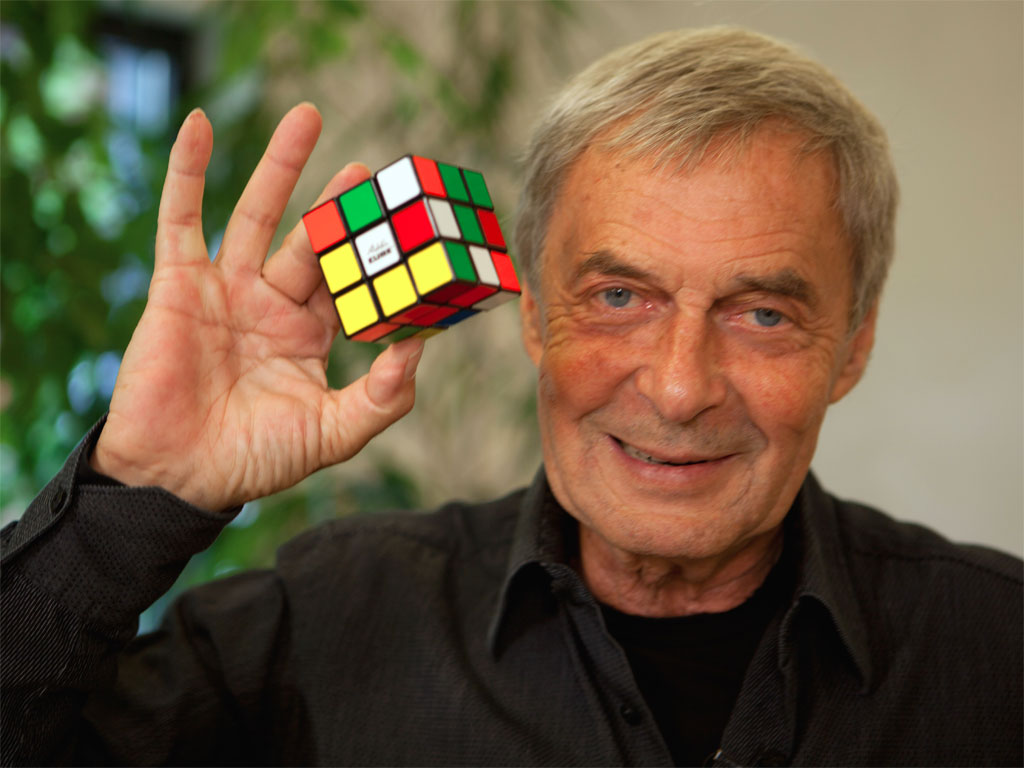
\includegraphics[scale=0.15]{erno.jpg}
	\caption{Ern\H{o} Rubik with his creation}
\end{figure}
\begin{figure}[h]
	\centering
	\begin{subfigure}[b]{0.3\textwidth}
		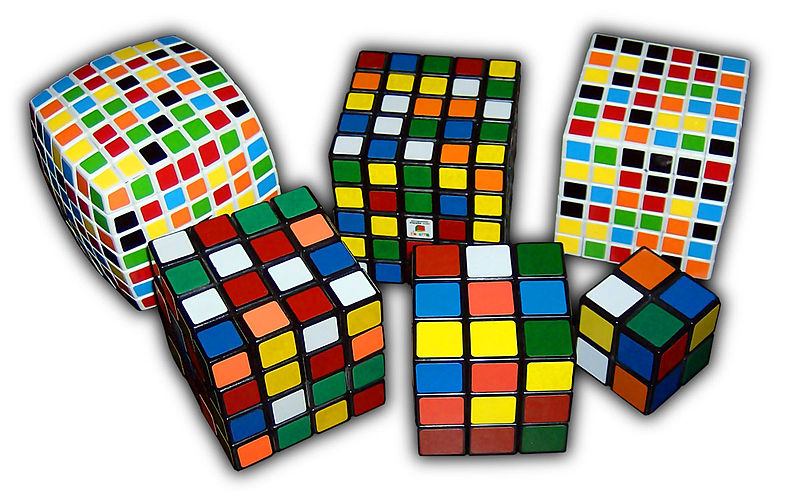
\includegraphics[width=\textwidth]{variants.jpg}
		\caption{Physical Cubes}
	\end{subfigure}\begin{subfigure}[b]{0.3\textwidth}
		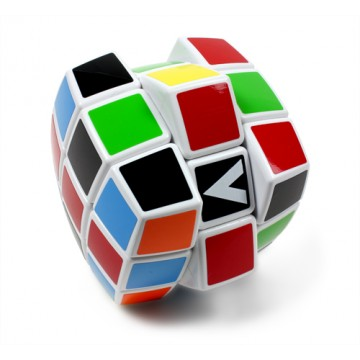
\includegraphics[width=\textwidth]{speed.jpg}	
		\caption{Professional `speedcube'}
	\end{subfigure}\begin{subfigure}[b]{0.3\textwidth}
		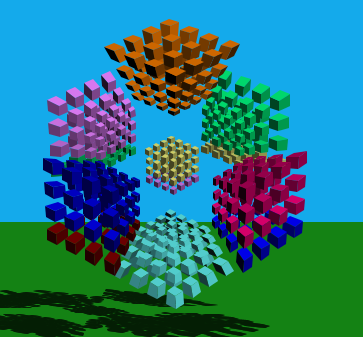
\includegraphics[width=\textwidth]{4d.png}
		\caption{Virtual $4{\times}4{\times}4{\times}4$  cube}	\end{subfigure}
	\caption{Cube variants}
\end{figure}	\newpage
	 An instant hit in the West, the cube became an icon of the '80s, inspiring a number of contests and clubs. It also spun-off a number of derivative puzzles, from the \cube{4} `Rubik's Revenge' to the \cube{17} `Over The Top'. Further, computer modelling has allowed enthusiasts to play with variants that would be impractical (hundreds or thousands of cubelets) or even impossible (higher-dimension cubes) to build in real life.
	
The standard cube is composed of 26 pieces, also called `cubelets':\begin{description}
	\item[6 Centre Pieces] These pieces are at the centres of the cube faces. They feature one colour each. As can be seen in Figure~\ref{fig:cutaway}, these pieces are always stationary relative to one another.
	\item[12 Edge Pieces] Edge pieces are located in between two centre faces. They have two colours each, which determine the final position of the piece\footnote{For example, in Figure~\ref{fig:cutaway}, the blue-orange edge would go between the blue and orange centres. Since blue and green are opposite to each other, there is no blue-green edge.}. These rotate around the centres.
	\item[8 Corner Pieces] These are located at the corners of the cube, and have three colours each. As with edge pieces, these colours determine the final position of the piece\footnote{The blue-orange-yellow corner goes between the blue, orange and yellow edges. There is no blue-orange green corner.}.
\end{description}
This gives a total of $6\times 1+12\times 2+8\times 3=9\times 6=54$ facelets.

\begin{figure}[h]
	\centering
		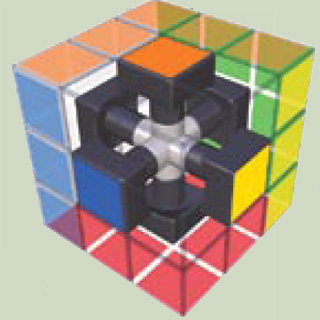
\includegraphics[scale=0.5]{cutaway.jpg}
	\caption{Cutaway Diagram}\label{fig:cutaway}
\end{figure}